\documentclass[UTF8]{ctexart}
\usepackage{ctex}
\usepackage[a4paper,left=2.5cm,right=2.5cm,top=2.5cm,bottom=2.5cm]{geometry}
\usepackage{enumerate}
\usepackage{balance}
\usepackage{fancyhdr}
\usepackage{xcolor}
\usepackage{zhlipsum}%乱字
\usepackage{amsmath}
\usepackage{pgfornament}
\usepackage{makeidx}
\makeindex
\usepackage{tabularx,booktabs}
\newcolumntype{Z}{>{\centering\arraybackslash}X}
\usepackage{dingbat,bbding}%铅笔手指宏包
\usepackage[thmmarks]{ntheorem}
{ % 利用分组, 格式设置只作用于证明环境
	\theoremstyle{nonumberplain}
	\theoremheaderfont{\bfseries}%最前面的粗体
	%\theorembodyfont{\fangsong}% \normalfont}%内容取消斜体
	%\theoremsymbol{\Square}
    %\newtheorem{solution}{\smallpencil}
    \newtheorem{Q}{Q:}
}
{ % 利用分组, 格式设置只作用于证明环境
	\theoremstyle{nonumberplain}
	\theoremheaderfont{\bfseries}%最前面的粗体
	%\theorembodyfont{\normalfont}%内容取消斜体
	\theoremsymbol{\Square}
    \newtheorem{A}{A:}
}
\newcommand{\FAQ}[2]{
    \begin{Q}
        #1
    \end{Q}
    \begin{A}
        #2
    \end{A}
}

\pagestyle{fancy}% 使用 fancy 风格
\fancyhf{} % 清除所有页眉页脚
\chead{\kaishu \itshape 江西理工大学常识FAQ}
\rhead{--\textit{\thepage/\pageref{LastPage}--}}
%\cfoot{\pgfornament{87}}
%\lhead{\textcolor{cyan}{\textit{sikouhjw}}}
\usepackage{hyperref}
\hypersetup{
    colorlinks=true,
    pdfstartview=Fit,
    pdftitle={江西理工大学常识FAQ},
    pdfauthor={死抠},
    pdfkeywords={常识,FAQ},
}
\begin{document}
    %\printindex
    \section{关于本文档}
    本文档最初的目的是为了解放重复性的解答他人问题这个行为, 答案不一定完全正确, 有错误可以反馈到我的邮箱489765924@qq.com, 本文档已上传至 \href{https://github.com/sikouhjw/jxustFAQ}{github} .

    \section{索引}

    \begin{center}
    \begin{tabularx}{\textwidth}{ZZZZZ}
        \hyperlink{1}{考试卷出法} & \hyperlink{2}{政治课复习重点} & \hyperlink{3}{学分} & \hyperlink{4}{校级公选课} & \hyperlink{5}{学位证}\\
        \hyperlink{6}{绩点} & \hyperlink{7}{重修} & \hyperlink{8}{数学竞赛} & \hyperlink{9}{数学建模竞赛} & \hyperlink{10}{学习资料} \\
        \hyperlink{11}{公众号} & & & & \\
    \end{tabularx}
    \end{center}
    
    % \begin{center}
    %     \rule{\textwidth}{.4pt}
    % \end{center}
    
    \section{正文}
    
    \FAQ{\hypertarget{1}{学姐, 考试卷是怎么出的?}}{
        教研室先出若干份卷子, 做成题库, 交给教务处, 到考试时, 教务处抽取其中一套作为考试卷(正考、补考是不同的卷子).
    }

    \FAQ{\hypertarget{2}{能不能把毛概复习重点划得再细一点?}}{
        不能, 老师划的重点应该都是题库里的题, 老师也是不知道这次是哪套卷子、什么题目的.
    }

    \FAQ{\hypertarget{3}{学姐, 综合素质学分、创新创业实践学分是干嘛用的?}}{
        毕业时所需修满综合素质学分 $3$ 分, 创新创业实践学分 $2$ 分.

        综合素质学分获取方式见附录~\ref{fl:1}
        
        总的来看, 大概就是四六级、二级、献血什么的加综合素质学分.

        创新创业实践学分获取方式见附录~\ref{fl:2}
        
        总的来看, 就是学科竞赛、科研、创新类活动等加创新创业实践学分, 当然比较好混分的
        就是参加竞赛拿成功参赛奖和参加由团委、学工部、教务处及创新创业学院组织的各类创新创业讲坛和讲座. 

        另外, 关于创新创业实践学分还有几点常识:
        \begin{enumerate}
            \item 获取的创新创业实践学分的超出部分可认定为综合素质学分. 
            
            意思就是搞竞赛或者其他创新类
            活动搞得厉害的人直接搞满5分就不用为了综合素质学分去献血啥的了.
            \item 学生所参加的创新创业实践取得优异成绩, 获取较高的创新创业学分, 在满足本专业人才培养方案规定创新创业学分的基础上, 超出的学分可以申请免修本专业选修专业课程一门, 学分折算为
            (创新创业学分:选修专业课学分=2:1), 免修课程不多于一门次. 
            
            意思就是多的创新创业实践学分可以去抵消一门选修课.
        \end{enumerate}
    }

    \FAQ{\hypertarget{4}{学姐, 校级公选课是干嘛的, 是不是每学期都要选啊?}}{
        校级公选课修得的学分是“独立的”\footnote{不计入学位证的绩点分, 不计入综测的平均绩点分}, 毕业要求是修满3分即可, 不需要每学期都选课, 只要修满3分就ok了, 另外选网课(尔雅老师)比较好, 只需要刷网课比较轻松.
    }

    \FAQ{\hypertarget{5}{学姐, 学位证要怎么拿?}}{
        大概能描述为: 在满足能毕业的基础上, 必修课和选修课\footnote{指专业选修课}平均绩点大于等于70分.

        若平均绩点小于70分, 有如下补救措施:
        \begin{enumerate}
            \item 毕业时或毕业后一年内参加全国硕士研究生统一入学考试取得入学资格, 并就读硕士研究生. 
            
            意思就是考上研或者二战上岸就能补救.
            \item 毕业前修学英语的非英语专业学生毕业前参加CET-4达到600分及以上、或CET-6达到425分及以上(体育、艺术类学生参加CET-4达到425分及以上); 
            英语专业学生毕业前参加CET-6达600分及以上, 或毕业前或毕业后一年内取得专业英语八级合格证书; 学其它语种的参照执行; 
            
            意思就是对于大多数专业来说, 过四级600或者六级425就能补救.
            \item 毕业前网考托福(TOEFLIBT)笔试成绩72分(总分120)及以上;
            \item 毕业前雅思(IELTS)笔试成绩6.0分(总分9.0)及以上;
            \item 毕业前纸质托福(TOEFLPaper-based TEST)笔试成绩520分(总分677)及以上;
            \item 毕业前参加A类学科竞赛获得省级一等奖、国家级二等奖及以上奖励, 或参加B类学科竞赛获得省级一等奖、国家级一等奖. 
            参加团体竞赛获奖的应为获奖证书排名前三名; 或其它方面业绩突出, 受到省级以上表彰. 
            
            意思就是搞竞赛拿省一后你就不用担心学位证了(前提是你能毕业).
        \end{enumerate}
    }

    \FAQ{\hypertarget{6}{学姐, 绩点怎么计算呀?}}{
        绩点计算公式在这里$\sim$
        \begin{equation*}
            \text{平均绩点}=\frac{\sum((\text{分数}-50)\times \text{学分})}{\sum\text{学分}}
        \end{equation*}
        当然这是默认你没挂科的情况, 如果你挂科了, 那一科按0算, 即 $0\times\text{学分}$

        举个例子8, 小明的成绩为高数100, 英语80, 线性代数95, 那么他的平均绩点为 $\frac{50\times 5.5+30\times 3+45\times 2}{5.5+3+2} = 43.33$ , 当然我们一般习惯在此基础上除10, 即4.33.
    }
    

    \FAQ{\hypertarget{7}{学姐, 重修是怎么样的呀?}}{
        重修的条件为: 本学期已开设的所有已修读过的课程(成绩 $<80$ 分).

        重修的费用: 50元. (相比其它学校来说很便宜了)

        重修的报名方式: 登录教务系统\url{http://jw.jxust.edu.cn/}

        具体的要求详见教务处发的文件, 这里再提一提某些课程的重修方式
        \begin{enumerate}
            \item 高数、线代、概率论、C语言、马原、思修、毛概、近现代史的重修为看网课的形式, 至于平时分怎么来的, 不太清楚.
            \item 英语的重修是分「跟班重修」和「单独开一个班重修」, 「单独开一个班重修」会开两个班(本部和黄金), 这两个班的时间会错开, 方便同学\hyperlink{1.1}{补}平时分
            
            平时分由到课率和作业决定, 通常只上五节课, 在周一至周五晚自习的时间上课, 一周一节, 给平时分的方式多种多样
            \begin{itemize}
                \item 刘书亮老师是用签到表签到, 当场做题作为作业, 签到一次14分, 作业做得好一次15分, 做得不好一次10分, 共5签到2作业, 即至少90分平时分, 只需卷面分40即可及格.
                \item 邵文轩老师是用点到和作业签到, 两次作业当场做(写了专业班级、名字、学号就给满分, 一排一排收, 没有让别人帮忙的可能), 三次是点一个人走一个人(第二节课快下课时, 因此课间溜过去就行), 平时分轻松满分, 卷面分只需33.3即可及格.
            \end{itemize}
            如果你有一堂课有事没来, 可以去另一个校区开设的重修班\hypertarget{1.1}{补}, 让那边的老师开证明即可.
        \end{enumerate}
    }

    \FAQ{\hypertarget{8}{学姐, 我想了解下数学竞赛, 能说说吗?}}{
        推荐搞数学竞赛的人走以下流程: 加入数学协会, 参加数学协会培训 $\to$ 参加路易杯\footnote{数学协会举办的私人性质比赛} $\to$ 参加校级竞赛 $\to$ 申请参加数学竞赛暑期培训 $\to$ 参加暑期培训并进行三次考试 $\to$ 申请报名CMC预赛 $\to$ $\begin{cases}
            \text{通过, 准备比赛}\\
            \text{没通过, 自费比赛}
        \end{cases}$ $\to$ 拿奖 $\to$ 从参加校赛开始重复以上流程

        这样下来一般人最多可以获得四次校一和三次省一
    }

    \FAQ{\hypertarget{9}{学姐, 我想了解下数学建模竞赛, 能说说吗?}}{
        首先自行去了解什么是「数学建模」, 然后再讲流程. 我校很特殊, 只允许在大二时参加高教社杯数学建模竞赛\footnote{即「国赛」}. 大二 $\to$ 加入数学建模协会 $\to$ 选择「数学建模」校级公选课\footnote{一定要加入协会, 不会直接在教务系统上选课, 而是在协会报名后从教务处那边录入}

        $\to$ $\begin{cases}
            \text{参加五一数学建模竞赛或其他比赛} & \text{可选}\\
            \text{只进行选修课} & \text{必走}
        \end{cases}$ $\to$ 参加校级数学建模比赛\footnote{2019年校赛: \url{https://www.zhihu.com/question/325608074/answer/695975094}} $\to$ 校赛答辩\footnote{问你是否参加暑期培训, 论文模型的思路等} $\to$ 综合各方面选拔出暑假培训人员 $\to$ 暑期培训 $\to$ 国赛
    }

    \FAQ{\hypertarget{10}{学姐, 到哪里可以找学习资料呀?}}{
        我将我收集整理的学习资料放在了github上, 链接
        \begin{center}
            \url{https://github.com/sikouhjw/jxust-Learning-database}
        \end{center}
    }

    \FAQ{\hypertarget{11}{学姐, 在哪里可以看学校、各个学院近期办的活动或者看优秀的学长学姐的考研/保研经历呀?}}{
        首先学校官网\url{http://www.jxust.cn/}还有各个学院的官网\footnote{这里再给出一个网站\url{http://www.jxust.cn/index/zbgg.htm}, 这是我们学校招标的网站, 主要是为了看一年发一次的月饼和粽子是什么馅}, 当然有些学院官网的新闻更新会比较慢, 下面给出学校和各个学院的官方微信公众号\footnote{顺序按首字母排序}
        \begin{center}
            \begin{tabularx}{\textwidth}{ZcZc}
                \toprule
                组织 & 公众号 & 组织 & 公众号\\
                \midrule
                电气学院 & 电小工 & 外语外贸学院 & 滴答外院\\
                信息学院 & 笃信好学自强不息 & 创新创业学院 & 江理双创\\
                学校 & 江西理工大学 & 学校 & 江西理工大学团委\\
                图书馆 & 江西理工大学图书馆 & 文法学院 & 江西理工大学文法学院\\
                机电学院 & 江西理工机电分团委 & 经管学院 & 江西理工经管学院分团委\\
                资环学院 & 江西理工资环学院团委 & 建测学院 & 建筑与测绘工程学院团委\\
                理学院 & 理学小阳 & 材料冶金化学学部 & 江理材料冶金化学学部\\
                \bottomrule
            \end{tabularx}
        \end{center}
        当然这里给出一些个人认为值得关注的公众号: 仍然在路上、共青团中央、江西共青团.
    }

    \newpage
    \appendix
    \section{综合素质学分认定标准表}\label{fl:1}
    \begin{center}
        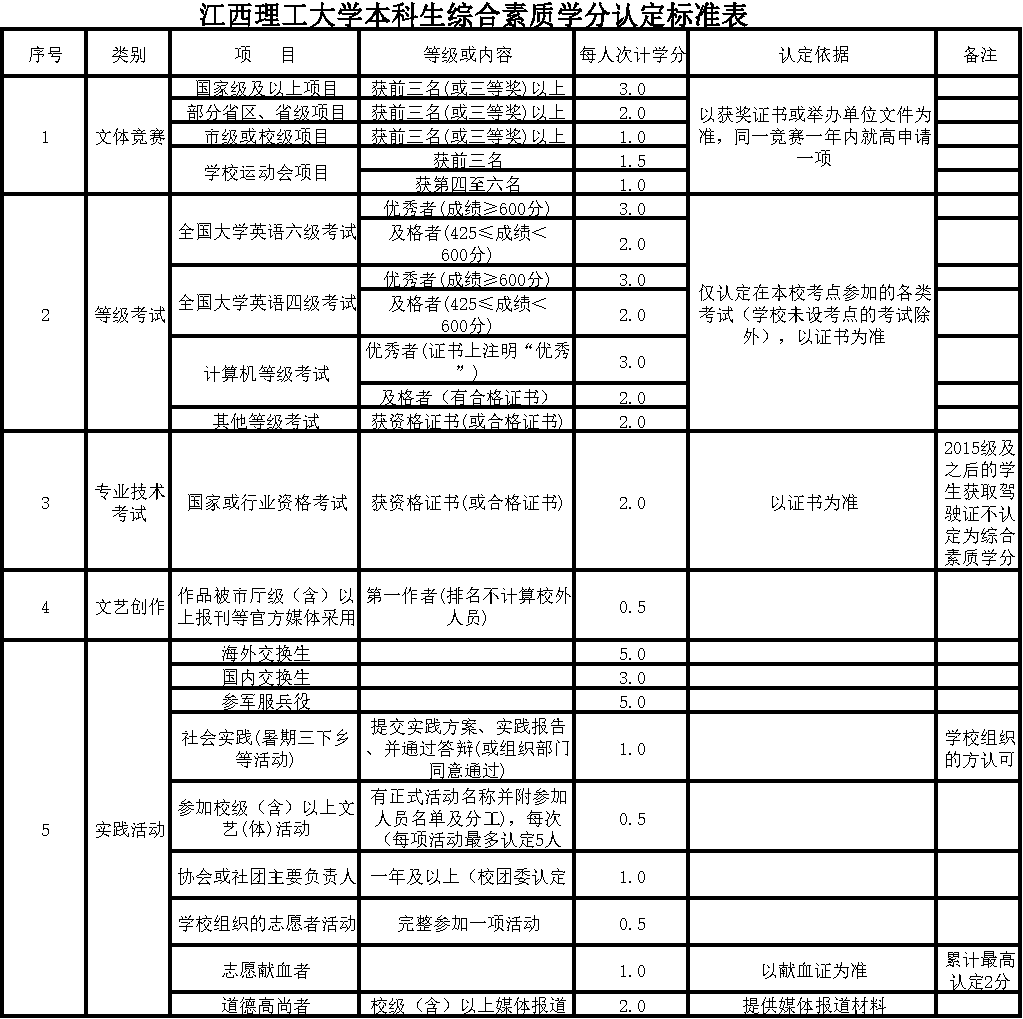
\includegraphics[width=\textwidth]{zhsz}
    \end{center}

    \section{创新创业实践学分}\label{fl:2}
    \begin{center}
        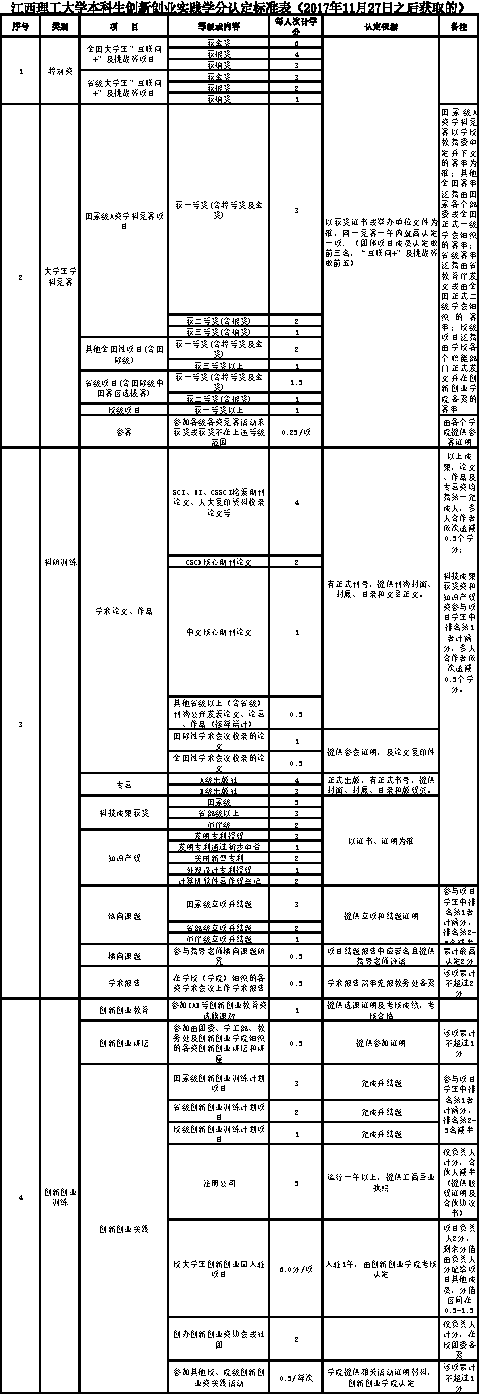
\includegraphics[height=0.8\textheight]{cxcy}
    \end{center}

\label{LastPage}
\end{document}